\documentclass[a4paper,norsk, 10pt]{article}
\usepackage[utf8]{inputenc}
\usepackage{verbatim}
\usepackage{listings}
\usepackage{graphicx}
\usepackage[norsk]{babel}
\usepackage{a4wide}
\usepackage{color}
\usepackage{amsmath}
\usepackage{float}
\usepackage{amssymb}
\usepackage[dvips]{epsfig}
\usepackage[toc,page]{appendix}
\usepackage[T1]{fontenc}
\usepackage{cite} % [2,3,4] --> [2--4]
\usepackage{shadow}
\usepackage{hyperref}
\usepackage{titling}
\usepackage{marvosym }
%\usepackage{subcaption}
\usepackage{subfig}
\usepackage[noabbrev]{cleveref}
\usepackage{cite}
\usepackage{todonotes}

\setlength{\droptitle}{-10em}   % This is your set screw

\setcounter{tocdepth}{2}

\lstset{language=c++}
\lstset{alsolanguage=[90]Fortran}
\lstset{alsolanguage=Python}
\lstset{basicstyle=\small}
\lstset{backgroundcolor=\color{white}}
\lstset{frame=single}
\lstset{stringstyle=\ttfamily}
\lstset{keywordstyle=\color{red}\bfseries}
\lstset{commentstyle=\itshape\color{blue}}
\lstset{showspaces=false}
\lstset{showstringspaces=false}
\lstset{showtabs=false}
\lstset{breaklines}
\title{AST5220 Milestone 3}
\author{Daniel Heinesen, daniehei}
\begin{document}
\maketitle

\section{Introduction}
In the previous milestones we found how the Universe expands, and how the coupling of electrons and photons influences the free mean path -- optical thickness $\tau$ -- of the photons. This means that we are ready to look at how initial perturbations in the Universe evolve. We will do this by integrating the Einstein-Boltzmann equations (see sec. \ref{sec:theory}) from an initial time deep in the radiation dominated era, well before decoupling, until today. Having integrated these equation for the scalar metric perturbations $\Phi$ and $\Psi$, the density perturbations of dark matter and baryons $\delta$ and $\delta_b$ and the velocity of dark matter and baryons $v$ and $v_b$, we can look at the different Fourier scales and learn how different scales are affected.

\section{Theory}\label{sec:theory}

\subsection{Normal Integration}\label{sec:normal}
We are interested in showing, given some initial conditions, how do perturbations evolve through time. by using Einstein's field equations and Boltzmann's equation

\begin{equation}
\frac{df}{dt} = C[f],
\end{equation}
where $f$ is the distribution of a given quantity and $C[f]$ is the collision term of the given distribution. The collection of coupled differential equations one gets from these expressions is called the Einstein-Boltzmann equations.

One can show that the Einstein-Boltzmann equation for the quantities we are interested in is given as

\begin{equation}
\Theta_0 ' = -\frac{ck}{\mathcal{H}}\Theta_1 - \Phi',
\end{equation}
\begin{equation}
\Theta_1' = \frac{ck}{3\mathcal{H}}\Theta_0 - \frac{2ck}{3\mathcal{H}}\Theta_2 + \frac{ck}{3\mathcal{H}}\Psi + \tau'\left[\Theta_1 + \frac{1}{3}v_b\right],
\end{equation}
\begin{equation}
\Theta_l' = \frac{lck}{(2l+1)\mathcal{H}}\Theta_{l-1} - \frac{(l+1)ck}{(2l+1)\mathcal{H}}\Theta_{l+1} + \tau'\left[\Theta_l - \frac{1}{10}\Theta_l \delta_{l,2}\right],\qquad 2 \leq l < l_{max}
\end{equation}
\begin{equation}
\Theta_l' = \frac{ck}{\mathcal{H}}\Theta_{l-1} - c\frac{l+1}{\mathcal{H}\eta(x)}\Theta_l + \tau'\Theta_l, \qquad l = l_{max}
\end{equation}
\begin{equation}
\delta' = \frac{ck}{\mathcal{H}}v - 3\Phi',
\end{equation}
\begin{equation}
v' = -v - \frac{ck}{\mathcal{H}}\Psi,
\end{equation}
\begin{equation}
\delta_b' = \frac{ck}{\mathcal{H}}v_b -3\Phi',
\end{equation}
\begin{equation}
v_b' = -v_b - \frac{ck}{\mathcal{H}}\Psi + \tau' R(3\Theta_1 + v_b),
\end{equation}
\begin{equation}
\Phi' = \Psi - \frac{c^2k^2}{3\mathcal{H}^2}\Phi + \frac{H_0^2}{2\mathcal{H}^2}\left[\Omega_ma^{-1}\delta + \Omega_b a^{-1}\delta_b + 4\Omega_r\Theta_0 a^{-2}\right],
\end{equation}
\begin{equation}
\Psi = -\Phi - \frac{12H_0^2}{c^2k^2a^2}\Omega_r\Theta_2,
\end{equation}
\begin{equation}
R = \frac{4\Omega_r}{3\Omega_b a},
\end{equation}
where $' = d/dx$, and $x = \ln a$ as in the previous milestones. All of the above equations are in Fourier space, with wave number $k$. This means that we can look at how the perturbations at different $k$ evolve (independently), which corresponds to different scales with $\lambda \propto k^{-1}$. We now have the differential equations we need to integrate, but to be able to do that we need initial conditions. We will start our integration a long time ago, when the particle horizon was extremely small compared to all $k$s, which means $k\eta << 1$. With this it is possible to get initial conditions as functions of $\Phi$
\begin{equation}
\Phi = 1,
\end{equation}
\begin{equation}
\delta = \delta_b = \frac{3}{2}\Phi,
\end{equation}
\begin{equation}
v = v_b = \frac{ck}{2\mathcal{H}}\Phi,
\end{equation}
\begin{equation}
\Theta_0 = \frac{1}{2}\Phi,
\end{equation}
\begin{equation}
\Theta_1 = -\frac{ck}{6\mathcal{H}}\Phi,
\end{equation}
\begin{equation}
\Theta_2 = -\frac{20ck}{45\mathcal{H}\tau'}\Theta_1,
\end{equation}
\begin{equation}
\Theta_l = -\frac{l}{2l+1}\frac{ck}{\mathcal{H}\tau'}\Theta_{l-1}.
\end{equation}
Just setting $\Phi = 1$ may seem odd, but we are through inflation only able to get the initial power spectrum of $\Phi$. But thankfully we do not need to worry about that before after we have integrated. We can, in other word, just set the initial value of $\Phi$ as we wish, integrate everything and then use the power spectrum of $\Phi$ after the integration. This gives the same result as if we would have gotten if we just the power spectrum as the initial value.

An other ting to notice is that we have defined a $l_{max}$, while $l$ in reality can take an infinite number of values. This is because we can use a technique called \textit{line of sight integration}, where only a small number of $l$s are needed to find the rest. This will be done in milestone 4, where we also will use the power spectrum of $\Phi$.


\subsection{Tight Coupling}\label{sec:tight}
There is one period we need to be careful of. At early times, before recombination, the mean free path of the photons are really small, meaning that $\tau >> 1$. During this time photons are unable to travel far before being scattered by electrons. This makes the photon aware only of a small area around it. This means that the baryons and photons are tightly coupled, behaving more like a single fluid. Due to the coupling, all but the largest perturbation are smoothed out, leaving the fluid in near equilibrium. All momentums of the photon temperatures are therefore negligible, except from $\Theta_0$ and $\Theta_1$. This is all well and fine, except from the fact that we now have a $\tau'$ which is very large multiplied with a factor $3\Theta_1-v_b$ which is very small, leading to numerical instability. This means that we need another way of integrating during this period. One can show that with these limitations we can integrate most of the expressions as before, but need to change $v_b'$ and $\Theta_0'$ to

\begin{equation}
v_b' = \frac{1}{1+R}\left[-v_b - \frac{ck}{\mathcal{H}}\Psi + R(q + \frac{ck}{\mathcal{H}}(-\Theta_0 + 2\Theta_2) - \frac{ck}{\mathcal{H}}\Psi)\right],
\end{equation}
\begin{equation}
\Theta_0' = \frac{1}{3}(q - v_b'),
\end{equation}
where 
\begin{equation}
q = \frac{-[(1-2R)\tau' + (1+R)\tau''](3\Theta_1 + v_b) - \frac{ck}{\mathcal{H}}\Psi + (1-\frac{\mathcal{H}'}{\mathcal{H}})\frac{ck}{\mathcal{H}}(-\Theta_0 + 2\Theta_2) - \frac{ck}{\mathcal{H}}\Theta_0'}{(1+R)\tau' + \frac{\mathcal{H}'}{\mathcal{H}} - 1}.
\end{equation}
With these we can calculate the other momenta as
\begin{equation}
\Theta_2 = \frac{-20ck}{45\mathcal{H}\tau'}\Theta_1,
\end{equation}
\begin{equation}
\Theta_l = -\frac{l}{2l+1}\frac{ck}{\mathcal{H}\tau'}\Theta_{l-1}
\end{equation}

So when will we use the tight coupling functions. We are going to define tight coupling as ending when either $|\tau'| < 10$, $\left|\frac{ck}{\mathcal{H}\tau'}\right|>0.1$ or recombination have started.

\section{Method}
Having the differential equations and initial values we can now begin to integrate. We want to integrate the equations from $x = \ln a_{init} = \ln 10^{-8}$ until today, where $x_0 = 0$. Since we know that different eras are more sensitive to numerical instability, we will make a x-grid with different step sizes. Before recombination we will have $1000$ grid points, during recombination we will use $200$ grid points, and $300$ grid points between the end of recombination and now. 

Since all the $k$s are independent, we can integrate them one by one. For this report only six such $k$s are used: $k = 0.1, 8.4, 85.9, 245.1, 636.8, 1000 H_0/c$\footnote{This choice was made so that it was possible to use the plots, published by the lecturer last year, as sanity checks.}. This is to demonstrate the physics at different scales. For the last milestone this will changed to $100$ values of $k$, distributed as given in Callin \cite{callin}

\begin{equation}
k_i = k_{min} + (k_{max}-k_{min})\cdot\left(\frac{i}{100}\right)^2.
\end{equation}

For each $k$ we start by finding at which value of $x$ tight coupling ends. We then use the the equations found in sec. \ref{sec:tight} during the integration. Note that only $\Theta_0$ and $\Theta_1$ are integrated here, the rest of the momenta are just algebraic expressions. When tight coupling is over, we can instead start to use the differential equations from sec. \ref{sec:normal}. 

All the integration is done by an integration function from \textit{Numerical Recipes} with a Bulirsch-Stoer stepper.

Since the $x$ value of the end of tight coupling is different for each $k$, this value has to be calculated for each $k$. Arrays with all the relevant quantities are saved after each step, for later use.

As a note on my own implementation: Even though it seemed that we were meant to use $x_t$ from $time\_mod$, I instead implemented an x-array inside $evolution\_mod$. The reason was that I remembered the array in $time\_mod$ after implementing the new array, and by then it has to much a hassle to change, since everything was working...

\section{Results and Discussion}




\begin{figure*}[!htbp]
\centering
\begin{tabular}{@{}ccc@{}}
\subfloat[This shows the evolution of the pertibutions of the dark matter.  We can see that for all $k$s, the perturbations are constant before entering the horizon. After entering the horizon all perturbations will grow. \label{fig:delta}]{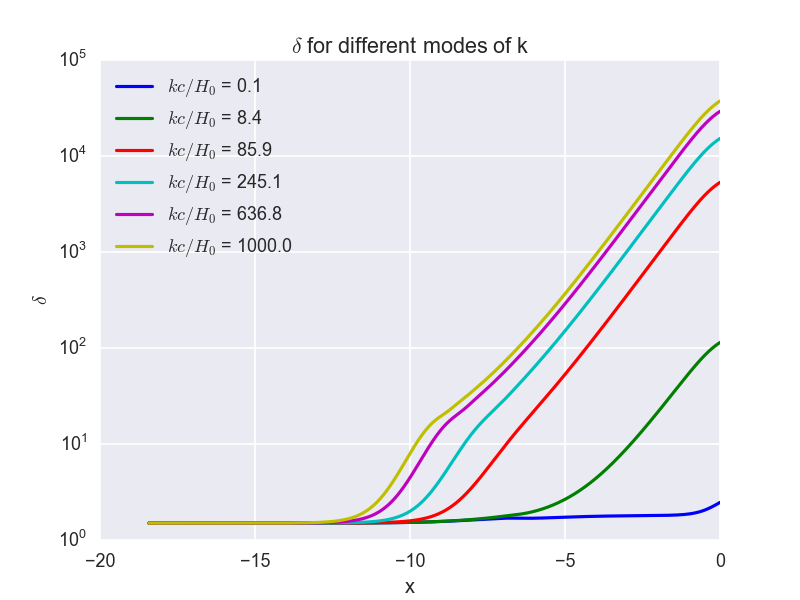
\includegraphics[width=0.5\textwidth]{delta.png}} & 
\subfloat[This shows the evolution of the pertibutions of the bayonic matter.  We can see that for all $k$s, the perturbations are constant before entering the horizon. Perturbations entering the before recombination will oscillate. These perturbations, and the parturbations entering after recombination, will start to grow after recombination. Many of the plots I have compared with have the spikes go further down. Since everything else works, I guess that this is just due to the $x$s I have used to plot.\label{fig:delta_b}]{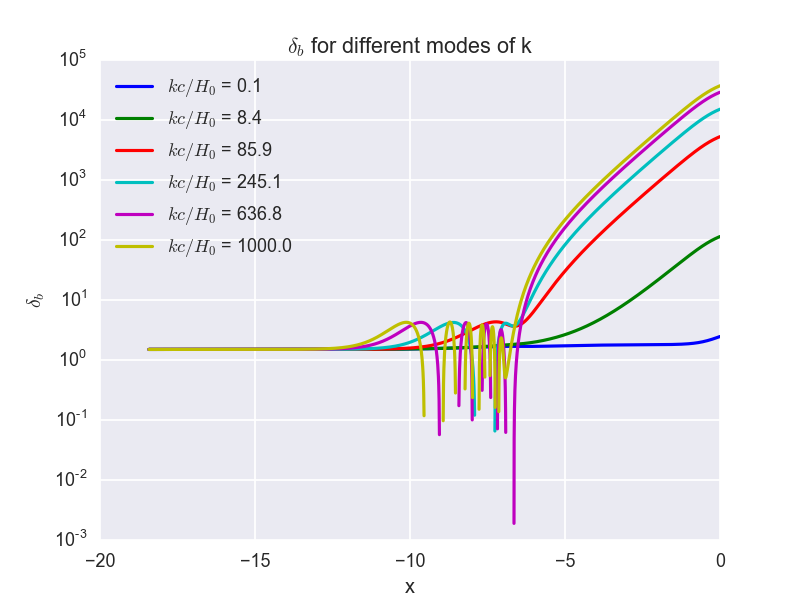
\includegraphics[width=0.5\textwidth]{delta_b.png}} \\
\subfloat[Velocity of dark matter. The velocity will more or less follow the growth in the dark matter perturbations.\label{fig:v}]{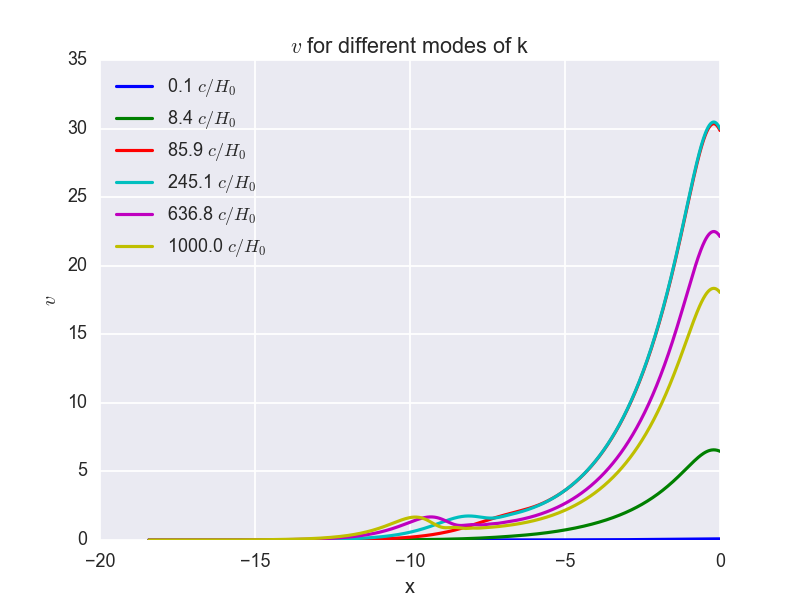
\includegraphics[width=0.5\textwidth]{v.png}} &
\subfloat[Velocity of baryonic matter. The velocity will more or less follow the growth in the baryonic matter perturbations\label{fig:v_b}]{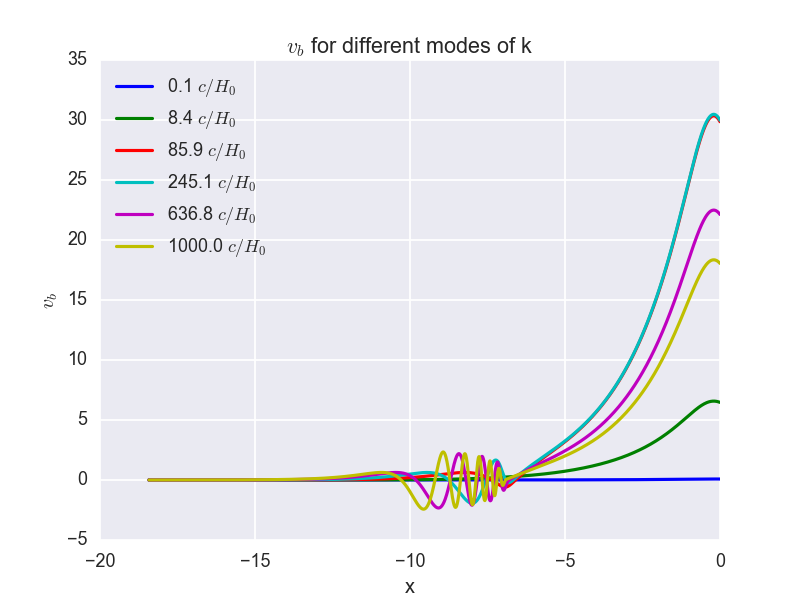
\includegraphics[width=0.5\textwidth]{v_b.png}} 
\end{tabular}
\caption[]{Plots showing the growth of the perturbations and the velocity of dark and baryonic matter. The different colors correspond to different $k$s, with higher values of $k$ corresponding to smaller scales.}
\label{fig:delta_v}
\end{figure*}


\begin{figure*}[!htbp]
\centering
\begin{tabular}{@{}ccc@{}}
\subfloat[The gravitational curvature potential $\Phi$. As with the matter, perturbations before entering the horizon are constant. The three larges $k$s (corresponding to smalles scales) will enter the horizon during radiation domination, rapidly decay before starting to oscillate. The oscillation will be dampend, and (after the start of matter domination) the potential will become constant. The largest scales will enter after radiation-matter equvalence, during which they will fall a bit and stay constant. Near present age, dark energy starts to dominate, and $\Phi$ starts to decrease.\label{fig:Phi}]{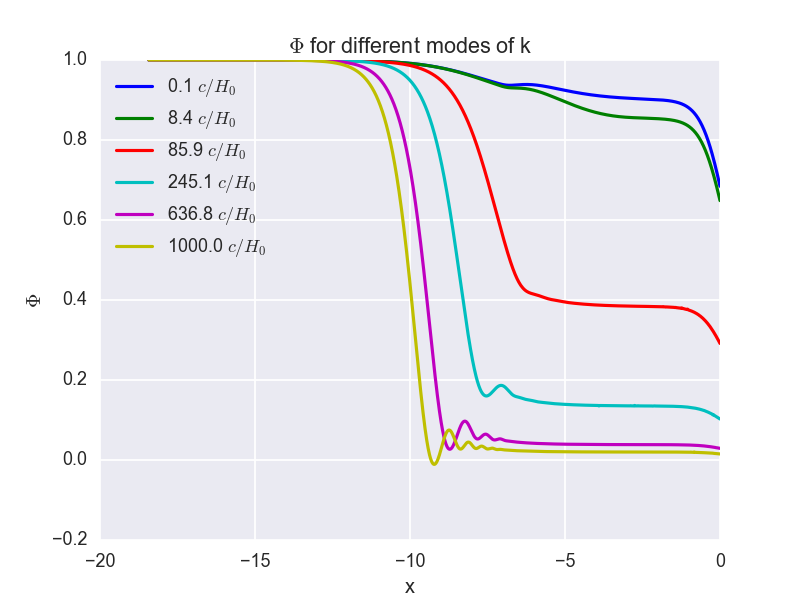
\includegraphics[width=0.5\textwidth]{Phi.png}} & 
\subfloat[The Newtonian potential $\Psi$. This growth more or less the same as $\Phi$ decreses. We can approximate that $\Psi = - \Phi$.\label{fig:Psi}]{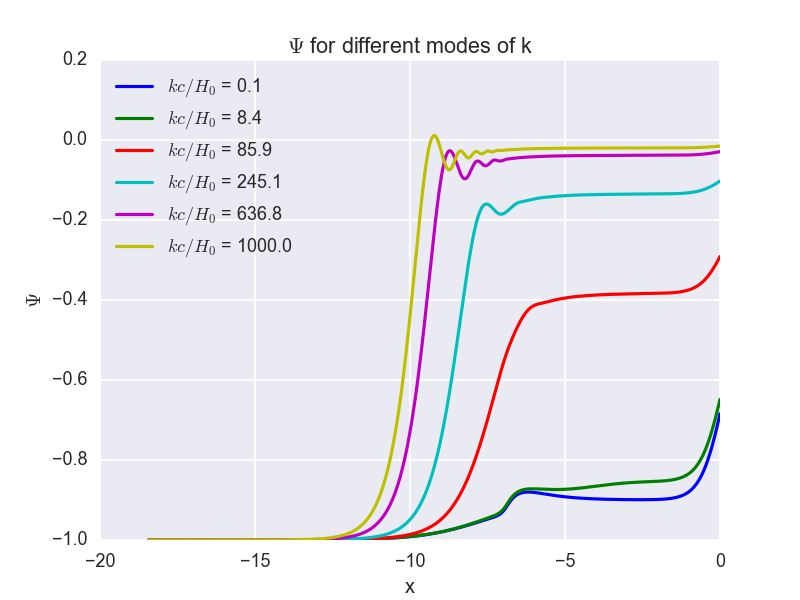
\includegraphics[width=0.5\textwidth]{Psi.png}} 
\end{tabular}
\caption[]{Plots showing the growth of the two gravitational potentials/perturbations. The different colors correspond to different $k$s, with higher values of $k$ corresponding to smaller scales.}
\label{fig:psi_phi}
\end{figure*}



\begin{figure}[!htbp]
\centering
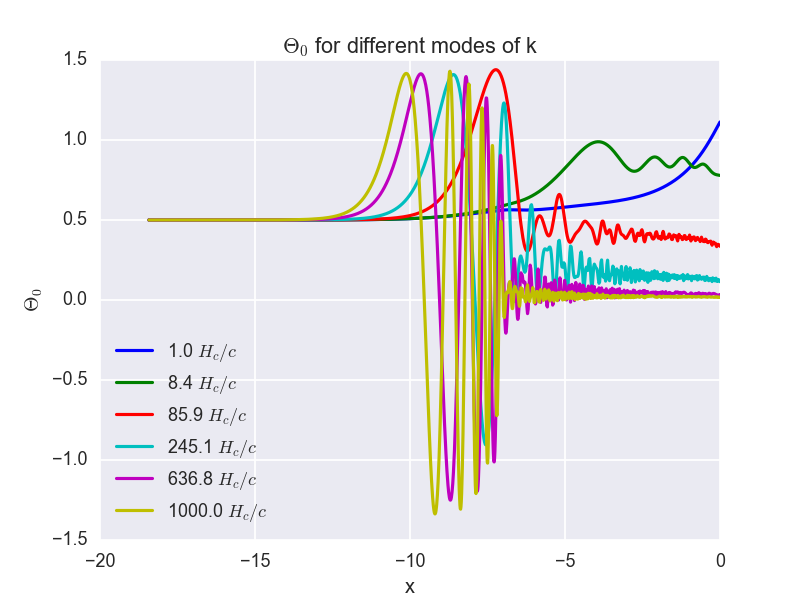
\includegraphics[scale=0.5]{Theta_0.png}
\caption{Growth of the zeroth momentum of the temperature for different $k$s. As the perturbations enter the horizon, they will start to fall into the gravitational well of dark matter together will baryonic matter, and oscillate. These oscillations are dampend and will start to die out.}\label{fig:theta}
\end{figure}




We'll start by looking at how the perturbations of matter evolves. If we look at fig. \ref{fig:delta} we see the perturbation of dark matter. Before a given scale has entered the horizon, it stays constant. There are two different eras a perturbation can enter the horizon: During radiation domination or during matter domination. The change from radiation to matter domination happens around $x\approx -8$ to $-9$. If a dark matter perturbation enters the horizon before this time, they will first start to grow, before being suppressed. This is what we can see in the figure for the largest values of $k$, which corresponds to the smallest scales -- those who will enter the horizon first. This suppression is a logarithmic growth. After matter starts to dominate, the suppression ends, and the growth will go as $\delta \propto a$. Larger scales (smaller $k$) will enter the horizon after the radiation domination, and will not be suppressed. They will instead always grow as $\delta \propto a$. \textit{Always} is of course a misnomer, since near present age dark energy will start to dominate. Things will then start to be pulled apart\todo{Will it?!}, making the perturbation of all scales start to flatten out. 

If we now look at the perturbations of baryonic matter, fig. \ref{fig:delta_b}, we see that the evolution shares many of the same characteristics, but upto $x \approx -7$ there are oscillations in the perturbation -- this again only applies to the small scales who have entered into the horizon by this time. This is due to the fact the the baryons are tightly couples to the photons, and thus we have a photon-baryon fluid. As this fluid falls into the dark matter gravity well, the radiation pressure will push the fluid apart, decreasing the perturbation. The pressure then decreases, and the fluid can collapse again. This happens over and over again, thus resulting in an oscillation. After recombination the baryons will no longer be affected by the radiation pressure, and are able to collapse. They will now collapse all on their own, but will fall into the gravitational wells made by the dark matter. This is why the perturbations for baryonic and dark matter evolves similarly after $x\approx -5$. The larger scale perturbations, who enters the horizon later will not have this oscillation, but will fall right into the gravity wells of the dark matter. We see the same slowing of growth near present age as we saw with dark matter.

The velocities of the dark and baryonic matter follow the perturbations. As a perturbation grows larger, the matter will fall faster, and vice versa. It is especially noticeable that during the oscillation of the baryons, their velocity oscillates as well. 

We can so look at the gravitational curvature potential $\Phi$ and Newtonian gravitational potential $\Psi$ in fig. \ref{fig:psi_phi}. Beginning with $\Phi$, fig. \ref{fig:Phi}, we see that, once again, the all the perturbations are constant before entering the horizon. The $k$s corresponding to the smallest scales will enter the horizon during radiation domination, and decay rapidly. They will so start to oscillate, as the photon-baryon fluid starts to oscillates. As the Universe becomes matter dominated, more specific dark matter dominated, $\Phi$ becomes determined more by the dark matter perturbations than by the photons. This means that the oscillation die out, since there are no oscillations in dark matter\todo{The dampening is also because of the expansion!}. We see that perturbations entering the horizon later will not oscillate as many times, before recombination ends and all oscillations stops. For the largest scale perturbations, they do not enter before after radiation domination. One can show that if a perturbation haven't entered the horizon before the age of radiation-matter equivalence, they will decrease by a factor $9/10$. During matter domination $\Phi$ on all scales will become constant, independently of when they entered the horizon. Again notice that as dark energy starts to dominate, $\Phi$ decreases.

$\Psi$ look more or less the same as $\Phi$, but where $\Phi$ decreases, $\Psi$ increases. A good approximation for $\Psi$ is $\Psi = - \Phi$.

The last figure, fig. \ref{fig:theta}, is of the zeroth momentum of the temperature $\Theta_0$. Again: All perturbations are constant before entering the horizon. We can see that when small scale perturbations grow when first entering the horizon, but as with $\Phi$ and $\delta_b$ they begin to oscillate. This is due to the gravitation and pressure of the photon-baryon fluid competing. After recombination the photons no longer are able to collapse with the baryons, and as the oscillations die out, the temperature perturbations become constant.


\newpage


\section{Conclusion}
We have now solved the Einstein-Boltzmann equations for different $k$s. We have also been able to use what we know about physics to interpret the different behaviours of the different quantities and scales. 

We saw that before entering the horizon $\delta$ was constant on all scales. Upon horizon entering, $\delta$ started to grow. The perturbations who entered during radiation domination was suppressed, but after matter domination all perturbations grew as $\delta \propto a$. $\delta_b$ followed $\delta$ during matter domination, but the perturbations that entered the horizon during radiation domination oscillated due to a tug-of-war between gravitation and radiation pressure. After decoupling, the baryons was unaffected by the radiation pressure, and began to settle into the gravitational well created by dark matter.
As the gravitational curvature potential $\Phi$ entered the horizon during radiation domination, it decreased rapidly before starting to oscillate with the baryons and photons. After the start of the matter domination, $\Phi$ on all scales became constant. The Newtonian potential $\Psi$ had more or less the same behaviour as $\Phi$ but in the other direction, so $\Psi \approx -\Phi$.
The perturbations of the photon temperature $\Theta_0$ who entered the horizon started to oscillated together with the baryons. After recombination, the temperature perturbations became more or less unaffected by the other constituents, and as the oscillations started to dampen, they became constant.

We can therefore soon reap the rewards of all our hard work, and calculate the CMB power spectrum!


\subsection{Notes on my own work}
For some reason my code is a bit slower than that of other people I've compared with. I have no idea why; I've used many hour trying to find the reason, and have even tried to use other people's code in the differentiation function, to see if that was the reason. But to no avail. So where other students code uses 2 min with $nk = 100$, by code used 5-10 min. I'll try to to find the reason before milestone 4, but as of now it is more of a nuisance than a real problem.

The report was some days late because of me feeling ill for most of the week. I hope this isn't that much reflected in the report...


\todo{Change temperature to temperature fluctuation!}
\todo{Change to \textit{Optical depth}}


\begin{thebibliography}{9}

\bibitem{callin}
  Callin, Peter,
  \textit{How to calculate the CMB spectrum},
  astro-ph/0606683
  2006.

\end{thebibliography}

\end{document}

